% Data flow diagram
% Author: David Fokkema
\documentclass{article}
\usepackage{tikz}
\usetikzlibrary{shapes,arrows}
\usepackage{pdflscape}
\usepackage[papersize={18cm, 8.5cm}, text={18cm, 8.5cm}]{geometry}
\usetikzlibrary{decorations.text}
\usepackage{xcolor}
% \selectcolormodel{gray}

\begin{document}
\thispagestyle{empty}
%\begin{landscape}
\begin{center}
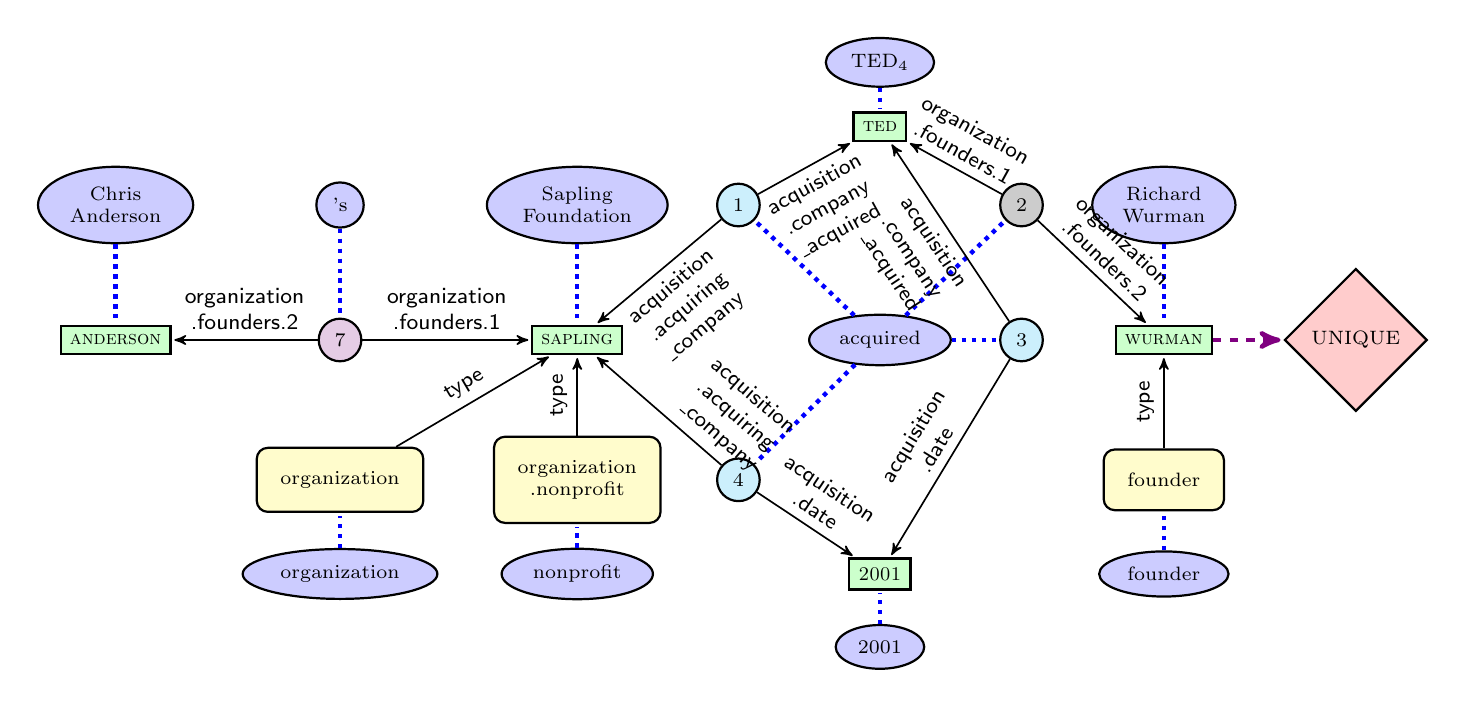
\begin{tikzpicture}[
  font=\sffamily,
  every matrix/.style={ampersand replacement=\&,column sep=0.6cm,row sep=0.3cm,font=\scriptsize},
  entity/.style={draw,thick,rectangle,fill=green!20},
  word/.style={draw,thick,ellipse,fill=blue!20},
  mediator/.style={draw,thick,circle},
  mediatorR/.style={draw,thick,circle,fill=cyan!20},
  mediatorV/.style={draw,thick,circle,fill=violet!20},
  mediatorY/.style={draw,thick,circle,fill=black!20},
  entityType/.style={draw,thick,rounded corners,fill=yellow!20,inner sep=.3cm},
  mathType/.style={draw,thick,diamond,fill=red!20},
  mediatorToEntity/.style={->,>=stealth',shorten >=1pt,semithick,black,sloped,above,font=\sffamily\footnotesize},
  typeToEntity/.style={->,>=stealth',shorten >=1pt,semithick,black,sloped,above,font=\sffamily\footnotesize},
  wordToEntity/.style={-,>=stealth',shorten >=1pt,ultra thick,dotted,blue,sloped,above,font=\sffamily\footnotesize},
  entityToMath/.style={->,>=stealth',shorten >=1pt,ultra thick,dashed,violet,sloped,above,font=\sffamily\footnotesize},
  every node/.style={align=center}]

  % Position the nodes using a matrix layout
  \matrix{ 
    \& \& \& \& \node[word] (wTED) {TED$_4$}; \\
    \& \& \& \& \node[entity] (eTED) {\textsc{ted}}; \\
    \node[word] (wAnderson) {Chris\\ Anderson}; \& \node[word] (wPos) {'s}; \& \node[word] (wSapling) {Sapling\\ Foundation}; \&  \node[mediatorR] (m1) {1}; \&  \& \node[mediatorY] (m2) {2}; \& \node[word] (wWurman) {Richard \\ Wurman};  \\
    \node[entity] (eAnderson) {\textsc{anderson}}; \& \node[mediatorV] (m3) {7}; \& \node[entity] (eSapling) {\textsc{sapling}}; \&   \& \node[word] (wAcquired) {acquired}; \& \node[mediatorR] (m4) {3}; \& \node[entity] (eWurman) {\textsc{wurman}}; \& \node[mathType] (mWurman) {UNIQUE}; \\
     \& \node[entityType] (tOrgan) {organization}; \& \node[entityType] (tProfit) {organization\\.nonprofit}; \&  \node[mediatorR] (m5) {4}; \& \&  \& \node[entityType] (tFounder) {founder}; \\
     \& \node[word] (wOrgan) {organization}; \& \node[word] (wProfit) {nonprofit}; \&  \& \node[entity] (e2001) {\textsc{2001}}; \& \& \node[word] (wFounder) {founder}; \\
     \& \&  \&  \& \node[word] (w2001) {2001}; \& \&  \\ 
  };
 
  
  
  % words to entities
  \draw [wordToEntity] (wAnderson) edge node {}  (eAnderson);
  \draw [wordToEntity] (wTED) edge node {}  (eTED);
  \draw [wordToEntity] (w2001) edge node {}  (e2001);
  \draw [wordToEntity] (wSapling) edge node {}  (eSapling);
  \draw [wordToEntity] (wWurman) edge node {}  (eWurman);
  % words to types
  \draw [wordToEntity] (wFounder) edge node {}  (tFounder);
  \draw [wordToEntity] (wOrgan) edge node {}  (tOrgan);
  \draw [wordToEntity] (wProfit) edge node {}  (tProfit);
  
  % event word to mediators
  \draw [wordToEntity] (wAcquired) edge node {}  (m1);
  \draw [wordToEntity] (wAcquired) edge node {}  (m2);
  \draw [wordToEntity] (wAcquired) edge node {}  (m4);
  \draw [wordToEntity] (wAcquired) edge node {}  (m5);
  \draw [wordToEntity] (wPos) edge node {}  (m3);
  
  % mediator to entities
  \draw [mediatorToEntity] (m1) edge node[below] {acquisition\\.company\\\_acquired}  (eTED);
  \draw [mediatorToEntity] (m1) edge node[below] {acquisition\\.acquiring\\\_company}  (eSapling);
  
  \draw [mediatorToEntity] (m2) edge node {organization\\.founders.1}  (eTED);
  \draw [mediatorToEntity] (m2) edge node {organization\\.founders.2}  (eWurman);
  
  \draw [mediatorToEntity] (m3) edge node {organization\\.founders.2}  (eAnderson);
  \draw [mediatorToEntity] (m3) edge node {organization\\.founders.1}  (eSapling);
  
  \draw [mediatorToEntity] (m4) edge node[below] {acquisition\\.company\\\_acquired}  (eTED);
  \draw [mediatorToEntity] (m4) edge node[above] {acquisition\\.date}  (e2001);
  
  \draw [mediatorToEntity] (m5) edge node[above right] {acquisition\\.acquiring\\\_company}  (eSapling);
  \draw [mediatorToEntity] (m5) edge node[above] {acquisition\\.date}  (e2001);
  
  % types to entities
  \draw [typeToEntity] (tOrgan) edge node {type}  (eSapling);
  \draw [typeToEntity] (tProfit) edge node {type}  (eSapling);
  \draw [typeToEntity] (tFounder) edge node {type}  (eWurman);
  
  % math func
  \draw [entityToMath] (eWurman) edge node {}  (mWurman);
  
\end{tikzpicture} 
\end{center}
% \end{landscape}

% \begin{tikzpicture}
% \node (One) at (-3,0) [shape=circle,draw] {$One$}; 
% \node (Two) at (3,0) [shape=circle,draw] {$Two$};
% \def\myshift#1{\raisebox{-2.5ex}}
% \draw [->,thick,postaction={decorate,decoration={text along path,text align=center,text={|\sffamily\myshift|Some more bent text}}}] (One) to [bend right=45]  (Two);
% \def\myshift#1{\raisebox{1ex}}
% \draw [->,thick,postaction={decorate,decoration={text along path,text align=center,text={|\sffamily\myshift|Some bent text}}}]      (One) to [bend left=45] (Two);
% \end{tikzpicture}


\end{document}
